
Uvrstimo zadane vrijednosti u $\vec{r}(t)$.
$$
\vec{r}(t)=(30ms^{-1}t) \vec{j} +(80m-\frac{1}{2}10ms^{-2}t^2 )\vec{k}
$$

\begin{enumerate}[label=\alph*)]
  \item $ \vec{r}(t=0,0s)=(30ms^{-1}0s) \vec{j} +(80m-\frac{1}{2}10ms^{-2}(0s)^2 )\vec{k}= 0m\vec{j}+80m\vec{k}$
  
  $ \vec{r}(t=0,5s)=(30ms^{-1}0,5s) \vec{j} +(80m-\frac{1}{2}10ms^{-2}(0,5s)^2 )\vec{k}= 15m\vec{j}+78,75m\vec{k}$
  
  $ \vec{r}(t=1,0s)=(30ms^{-1}1,0s) \vec{j} +(80m-\frac{1}{2}10ms^{-2}(1,0s)^2 )\vec{k}= 30m\vec{j}+75m\vec{k}$
  
  $ \vec{r}(t=1,5s)=(30ms^{-1}1,5s) \vec{j} +(80m-\frac{1}{2}10ms^{-2}(1,5s)^2 )\vec{k}= 45m\vec{j}+68,75m\vec{k}$
  
  $ \vec{r}(t=2,0s)=(30ms^{-1}2,0s) \vec{j} +(80m-\frac{1}{2}10ms^{-2}(2,0s)^2 )\vec{k}= 60m\vec{j}+60m\vec{k}$
  
  $ \vec{r}(t=2,5s)=(30ms^{-1}2,5s) \vec{j} +(80m-\frac{1}{2}10ms^{-2}(2,5s)^2 )\vec{k}= 75m\vec{j}+48,75m\vec{k}$
   
  $ \vec{r}(t=3,0s)=(30ms^{-1}3,0s) \vec{j} +(80m-\frac{1}{2}10ms^{-2}(3,0s)^2 )\vec{k}= 90m\vec{j}+35m\vec{k}$
  
  $ \vec{r}(t=3,5s)=(30ms^{-1}3,5s) \vec{j} +(80m-\frac{1}{2}10ms^{-2}(3,5s)^2 )\vec{k}= 105m\vec{j}+18,75m\vec{k}$

  $ \vec{r}(t=4,0s)=(30ms^{-1}4,0s) \vec{j} +(80m-\frac{1}{2}10ms^{-2}(4,0s)^2 )\vec{k}= 120m\vec{j}+0m\vec{k}$

\begin{figure}
%\begin{subfigure}{.5\textwidth}
  \centering
  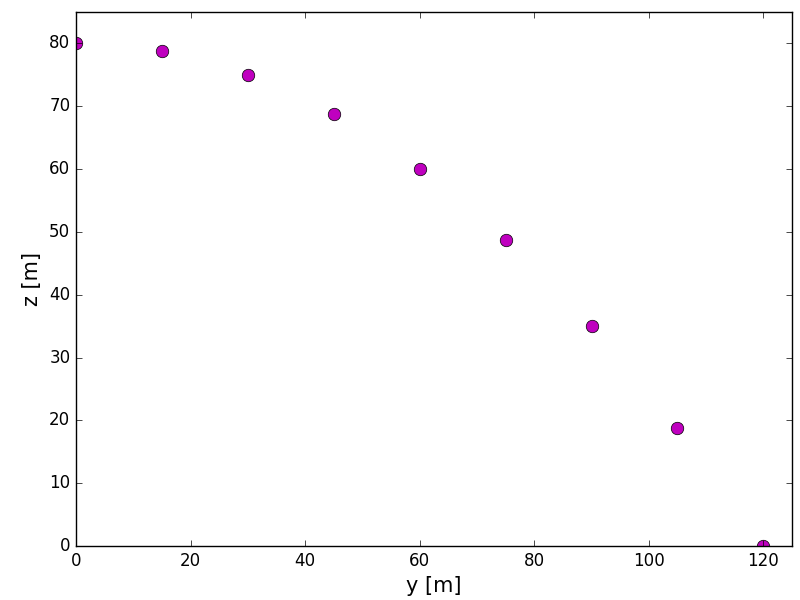
\includegraphics[width=0.5\linewidth]{Kinematika_materijalne_tocke/polozaj_MT.png}
%  \caption{1a}
%  \label{fig:sfig1}
%\end{subfigure}%
%\begin{subfigure}{.5\textwidth}
  \centering
  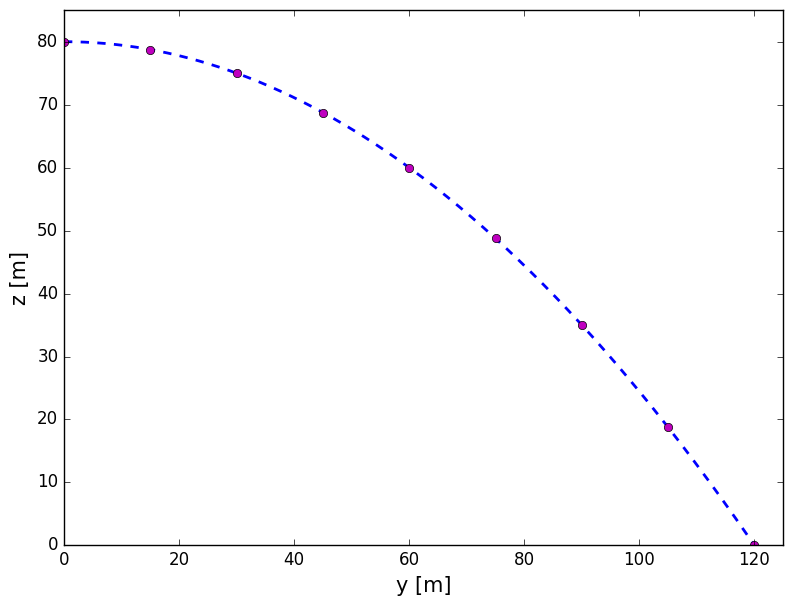
\includegraphics[width=.5\linewidth]{Kinematika_materijalne_tocke/krivulja_MT.png}
%  \caption{1b}
%  \label{fig:sfig2}
%\end{subfigure}
\caption{\textit{(lijevo)} Položaj MT za svakih $0,5\ s$. \textit{(desno)} Putanja MT do udarca o tlo.}
%\label{fig:poloza_MT}
\end{figure}
 
 
 
 \item $$\vec{v}(t)  = \frac{d\vec{r}(t)}{dt}$$
  
 $$\vec{v}(t)  = \frac{d}{dt} \left(z_0 \vec{k}+v_0t \vec{j}-\frac{1}{2}gt^2\vec{k}  \right)$$

 $$\vec{v}(t)  = v_0\vec{j}-gt\vec{k}$$
 
 \item $\vec{v}(t)  =30\ ms^{-1}\vec{j}-10\ ms^{-2}t\vec{k}$
 
 $\vec{v}(t=1s)  =30\ ms^{-1}\vec{j}-10\ ms^{-2}1s\vec{k}$
 
 $\vec{v}(t=1s)  =30\ ms^{-1}\vec{j}-10\ ms^{-1}\vec{k}$
 
 $\vec{v}(t=2s)  =30\ ms^{-1}\vec{j}-20\ ms^{-1}\vec{k}$
 
 $\vec{v}(t=3s)  =30\ ms^{-1}\vec{j}-30\ ms^{-1}\vec{k}$
  
 $\vec{v}(t=4s)  =30\ ms^{-1}\vec{j}-40\ ms^{-1}\vec{k}$
 
\begin{figure}
%\begin{subfigure}{.5\textwidth}
  \centering
  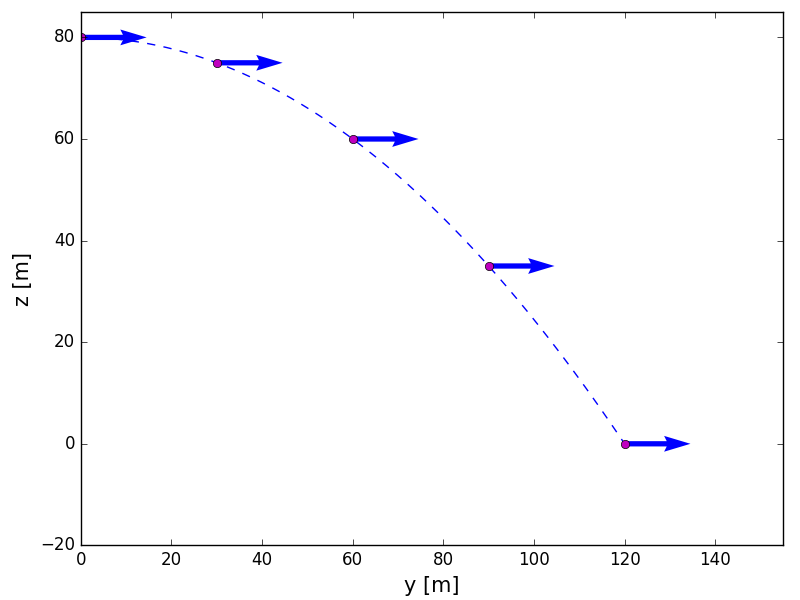
\includegraphics[width=0.4\linewidth]{Kinematika_materijalne_tocke/brzina_y.png}
%  \caption{1a}
%  \label{fig:sfig1}
%\end{subfigure}%
%\begin{subfigure}{.5\textwidth}
  \centering
  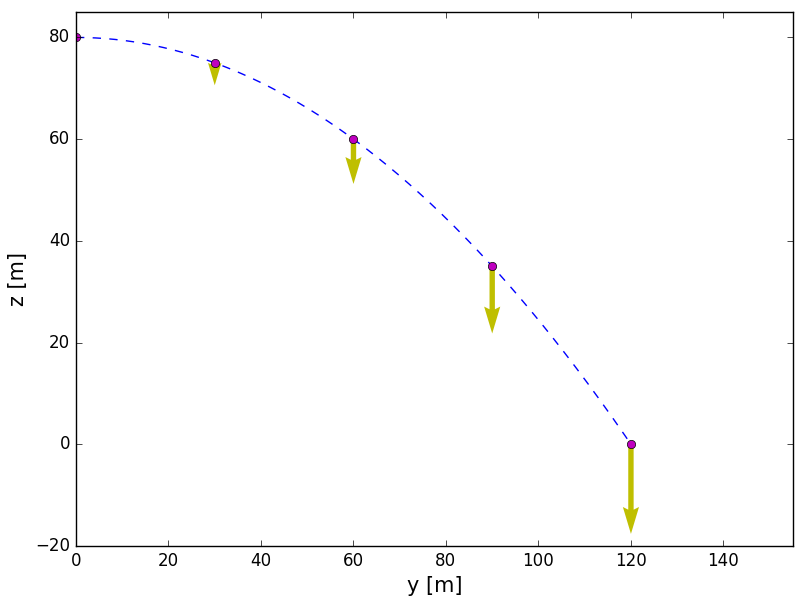
\includegraphics[width=.4\linewidth]{Kinematika_materijalne_tocke/brzina_z.png}
%  \caption{1b}
%  \label{fig:sfig2}
%\end{subfigure}
\centering
  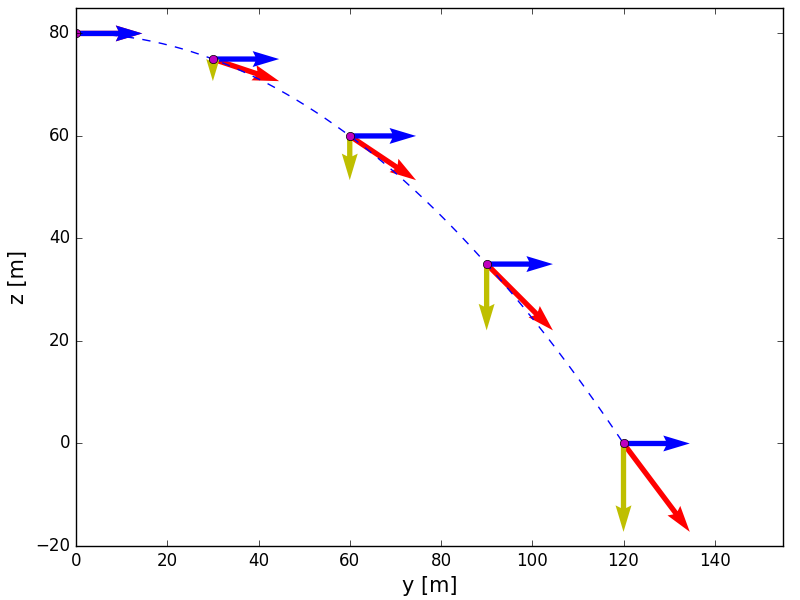
\includegraphics[width=.5\linewidth]{Kinematika_materijalne_tocke/brzina_ukupna.png}
\caption{\textit{(gore-lijevo)} Komponenta brzine u $y$-smjeru. \textit{(gore-desno)} Komponenta brzine u $z$-smjeru.\textit{(dolje)} Brzina tijela s komponentama.}
%\label{fig:brzina}
\end{figure}

$|\vec{v}(t=1s)|  = \sqrt{ (30\ ms^{-1})^2 + (-10\ ms^{-1})^2 } = 31,623\ ms^{-1} $

$|\vec{v}(t=2s)|  = \sqrt{ (30\ ms^{-1})^2 + (-20\ ms^{-1})^2 } = 36,055\ ms^{-1}  $

$|\vec{v}(t=3s)|  = \sqrt{ (30\ ms^{-1})^2 + (-30\ ms^{-1})^2 } = 42,43\ ms^{-1}  $

$|\vec{v}(t=4s)|  = \sqrt{ (30\ ms^{-1})^2 + (-40\ ms^{-1})^2 } = 50,0\ ms^{-1}  $


\item $$\vec{a}(t)  = \frac{d^2\vec{r}(t)}{dt^2}=\frac{d\vec{v}}{dt}$$
$$\vec{a}(t)  = \frac{d} {dt} \left( v_0\vec{j}-gt\vec{k}  \right)$$
$$ \vec{a}(t)  =  -g\vec{k}=-9,81\ ms^{-2}\vec{k}\approx -10\ ms^{-2}\vec{k} $$

\end{enumerate}
